\documentclass{beamer}
\usepackage{subfig}
\usepackage{epigraph} 
\usetheme{Madrid}
\usecolortheme{default}

%Information to be included in the title page:
\title{Changes in Drug Laws and College Enrollment}
\author{Ray Huang}
\institute{Senior Thesis}
\date{December 7, 2022}

\begin{document}

\frame{\titlepage}

%------------------------------------------------------------

\begin{frame}
\frametitle{Motivation}
\begin{quote}
  There’s 2.2 million people in the American prison system, and half a million of those are locked up for drug offenses. A lot of them were in the same boat as me: victims of the mandatory minimum... It’s the reason hundreds of thousands of nonviolent people—mostly black and brown people-- are rotting in prison. Rotting like the baloney and cheese sandwiches they serve for breakfast, lunch, and dinner...

  I’d been in prison for ten years by the time my petition reached the Supreme Court.
\end{quote}
\hspace*{\fill} - John Gargano, HONY
\end{frame}

%------------------------------------------------------------

\begin{frame}
\frametitle{Background I}
\begin{itemize}
    \item Anti-Drug Abuse Act of 1986 established mandatory sentencing minimums (with disparities across drugs)
    \begin{itemize}
        \item Increase in average time imprisoned for drug crimes from 22 months to 33 months
        \item Number of black people sent to federal prison skyrocketed from approximately 50 to 250 in 100,000 adults (Equal Justice Initiative)
    \end{itemize}
    \item Fair Sentencing Act of 2010 reduced disparities in sentencing and eliminated mandatory minimums
    \item Disparities in college attainment across race and gender have maintained across time
\end{itemize}
\end{frame}

%------------------------------------------------------------

\begin{frame}{Background II}
    \begin{figure}%
    \centering
    \subfloat[\centering College enrollment rates]{{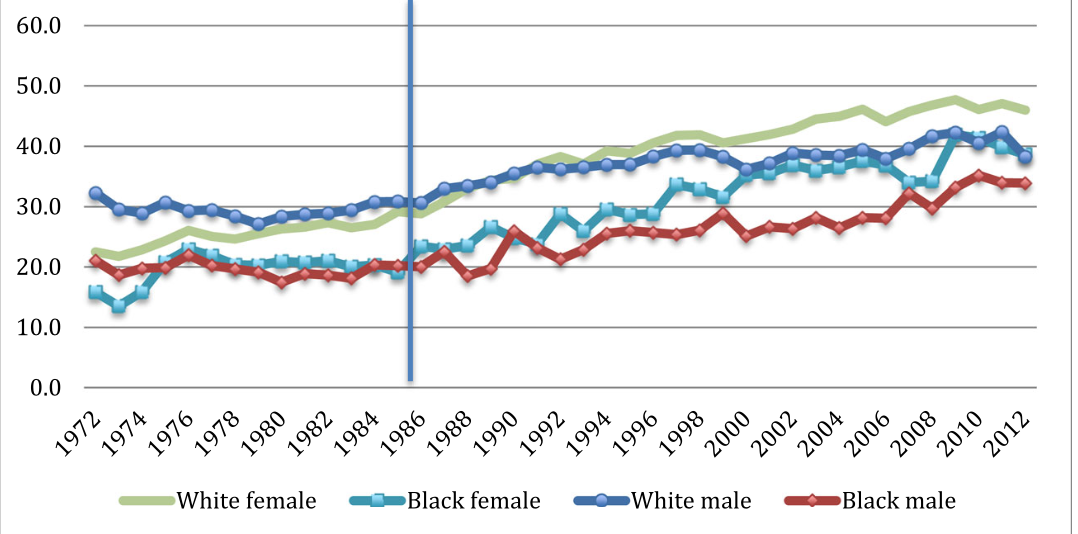
\includegraphics[width=5cm]{britton_fig1.png} }}%
    \qquad
    \subfloat[\centering Drug possession arrest rate (per 100,000)]{{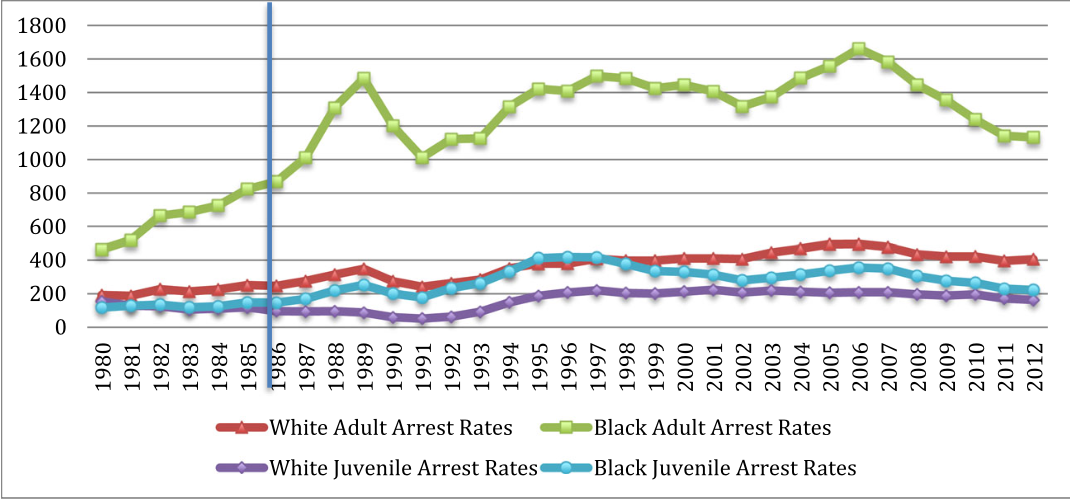
\includegraphics[width=5cm]{britton_fig2.png} }}%
    \caption{Education and possession trends over time (Britton, 2022)}
    \label{fig:example}%
\end{figure}
\end{frame}

%------------------------------------------------------------

\begin{frame}{Research questions}
    \begin{enumerate}
        \item Did the passage of the federal Anti-Drug Abuse Act of 1986 cause a fall in relative college enrollment for Black male students?
        \item Did the passage of the federal Fair Sentencing Act of 2010 cause an increase in relative college enrollment for Black male students?
    \end{enumerate}
\end{frame}

%------------------------------------------------------------

\begin{frame}
\frametitle{Data sources}
\begin{itemize}
  \item October Current Population Survey (CPS) education supplements 1982-2020
  \begin{itemize}
      \item Limitations: i) excludes incarcerated persons ii) cannot track movement across states
  \end{itemize}
  \item FBI Uniform Crime Reporting (UCR)
  \item Data on state-level possession/distribution penalties are manually collected from government publications
\end{itemize}
\end{frame}

%------------------------------------------------------------

\begin{frame}
\frametitle{1986 sample}
\begin{table}[htbp]\tiny
\centering
\caption{Summary Statistics}
\begin{tabular}{l*{2}{c}}
\hline\hline
                    &\multicolumn{1}{c}{(1)}&\multicolumn{1}{c}{(2)}\\
                    &\multicolumn{1}{c}{Pre-period}&\multicolumn{1}{c}{Post-period}\\
\hline
Male                &        0.49&        0.49\\
                    &     (0.500)&     (0.500)\\
[1em]
Black               &        0.14&        0.14\\
                    &     (0.346)&     (0.347)\\
[1em]
HS Graduate         &        0.82&        0.81\\
                    &     (0.385)&     (0.389)\\
[1em]
Enrolled in college &        0.24&        0.29\\
                    &     (0.426)&     (0.453)\\
[1em]
Enrolled in 4-year coll.&        0.24&        0.28\\
                    &     (0.426)&     (0.449)\\
\hline
Observations        &       47595&       79894\\
\hline\hline
\multicolumn{3}{l}{\footnotesize mean coefficients; sd in parentheses}\\
\end{tabular}
\end{table}

\end{frame}

%------------------------------------------------------------

\begin{frame}
\frametitle{Empirical strategy}
\begin{itemize}
    \item Baseline approach: using young white males and young black females as counterfactuals
    \item Can we leverage variation in state-level laws and drug usage/arrest rates improve the robustness of our results?
\end{itemize}
\end{frame}

%------------------------------------------------------------

\begin{frame}
\frametitle{Pre-trends}
\begin{center}
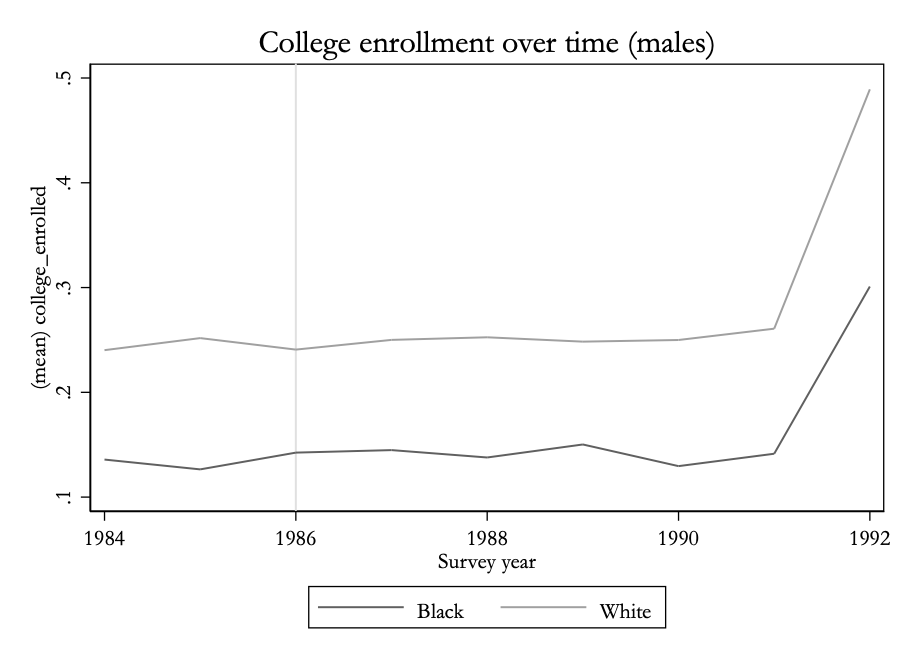
\includegraphics[width=.4\textwidth]{college_enroll_byrace_1986.png}
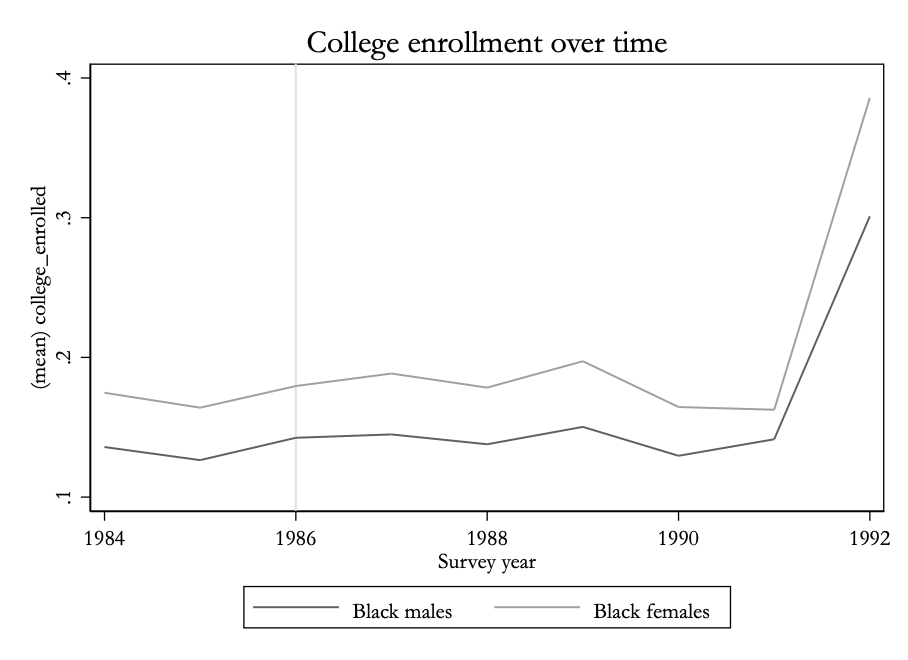
\includegraphics[width=.4\textwidth]{college_enroll_bysex_1986.png}
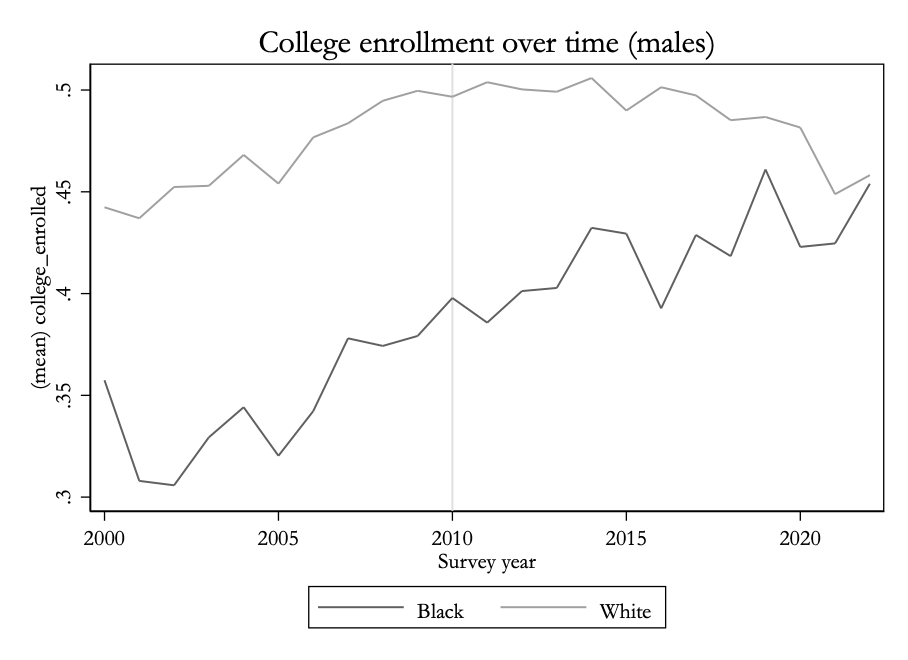
\includegraphics[width=.4\textwidth]{college_enroll_byrace_2010.png}
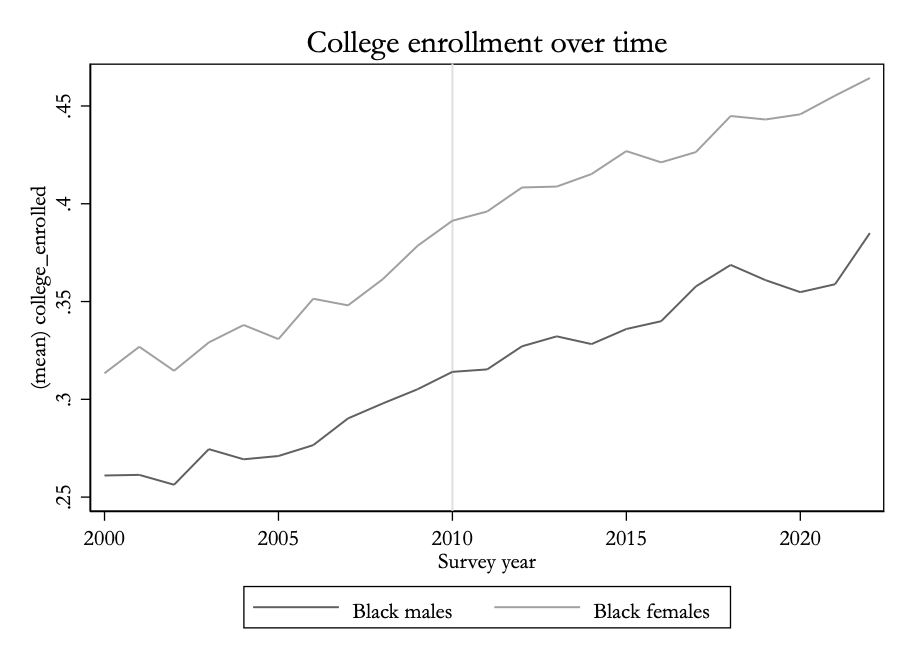
\includegraphics[width=.4\textwidth]{college_enroll_bysex_2010.png}
\end{center} 
\end{frame}

%------------------------------------------------------------

\begin{frame}
\frametitle{DiD results I, Anti-Drug Abuse Act}
\begin{table}[htbp]\centering
\def\sym#1{\ifmmode^{#1}\else\(^{#1}\)\fi}
\caption{Britton T2, DiD Impact of 1986 Act using white males}
\begin{tabular}{l*{3}{c}}
\hline\hline
                    &\multicolumn{1}{c}{(1)}         &\multicolumn{1}{c}{(2)}         &\multicolumn{1}{c}{(3)}         \\
\hline
after1986           &       .0369\sym{***}&      .01522\sym{**} &           0         \\
                    &   (.007408)         &   (.005981)         &         (.)         \\
[1em]
Black               &     -.09715\sym{***}&     -.05948\sym{***}&     -.05466\sym{***}\\
                    &    (.01181)         &    (.01025)         &    (.01083)         \\
[1em]
interaction         &     -.02207\sym{*}  &     -.02106\sym{*}  &     -.01981\sym{*}  \\
                    &    (.01175)         &    (.01143)         &     (.0113)         \\
[1em]
Constant            &       .2928\sym{***}&      -3.183\sym{***}&      -3.175\sym{***}\\
                    &   (.008707)         &     (.3267)         &     (.3309)         \\
\hline
Observations        &       56931         &       56931         &       56931         \\
Adjusted \(R^{2}\)  &       0.008         &       0.102         &       0.106         \\
State\_yr\_FE         &           N         &           N         &           Y         \\
Demographic\_controls&           N         &           Y         &           Y         \\
\tabnotes{3}{Estimates weighted using CPS October supplement weights. Robust standard errors clustered at state level. Controls: age, age-squared, Latino ethnicity, yearly state average unemployment rates, and (binned) family income.}

\end{frame}

%------------------------------------------------------------

\begin{frame}
\frametitle{DiD results II, Fair Sentencing Act}


\begin{table}[htbp]\centering
\def\sym#1{\ifmmode^{#1}\else\(^{#1}\)\fi}
\caption{Impact of the Fair Sentencing Act on College Enrollment: DiD Estimates Comparing Black and White Males}
\begin{tabular}{l*{3}{c}}
\hline\hline
                    &\multicolumn{1}{c}{(1)}         &\multicolumn{1}{c}{(2)}         &\multicolumn{1}{c}{(3)}         \\
\hline
Post-2010           &       .4605\sym{***}&       .1655\sym{***}&           0         \\
                    &   (.007575)         &    (.00999)         &         (.)         \\
[1em]
Black               &     -.04992\sym{***}&    -.007978         &    -.006736         \\
                    &   (.006469)         &   (.006119)         &     (.0061)         \\
[1em]
Post-2010 X Black   &     -.04527\sym{***}&     -.06463\sym{***}&     -.06378\sym{***}\\
                    &    (.01473)         &    (.01645)         &    (.01639)         \\
[1em]
Constant            &       .1649\sym{***}&      -.9772\sym{***}&      -.6099\sym{***}\\
                    &   (.004676)         &    (.01645)         &    (.02007)         \\
\hline
Observations        &      126471         &      126471         &      126471         \\
Adjusted \(R^{2}\)  &       0.216         &       0.304         &       0.323         \\
FE                  &           N         &           N         &           Y         \\
Controls            &           N         &           Y         &           Y         \\
\hline\hline
\multicolumn{4}{l}{\footnotesize Standard errors in parentheses}\\
\multicolumn{4}{l}{\footnotesize \sym{*} \(p<0.10\), \sym{**} \(p<0.05\), \sym{***} \(p<0.01\)}\\
\end{tabular}
\end{table}

\end{frame}

%------------------------------------------------------------

\begin{frame}
\frametitle{Further work}
\begin{itemize}
    \item Overall, the results so far are encouraging but far from robust (sensitive to specifications, weights, dropped observations, counterfactual group, etc)
    \item Further test the robustness of the DiD estimates
    \item Implement the DDIV / DDD approaches (similar to strategy implemented in Duflo, 2001)
    \item Can we use the same empirical approach to study the impact of these laws on other outcomes?
\end{itemize}
\end{frame}

%------------------------------------------------------------

\begin{frame}
\frametitle{Pre-trends (DDIV)}
Are states that did not increase the punitiveness of their drug laws a valid counterfactual?
\begin{figure}%
    \centering
    \subfloat[\centering]{{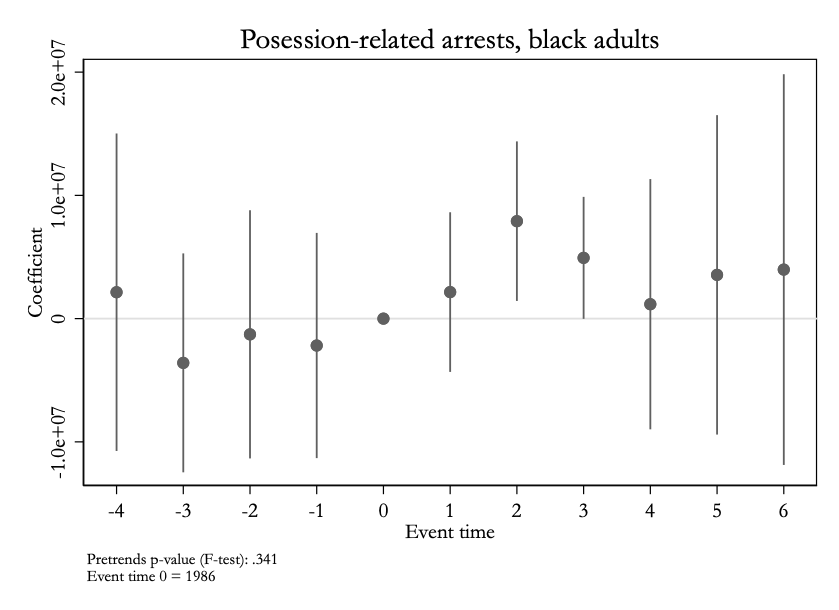
\includegraphics[width=5cm]{eventstudy_black.png} }}%
    \qquad
    \subfloat[\centering]{{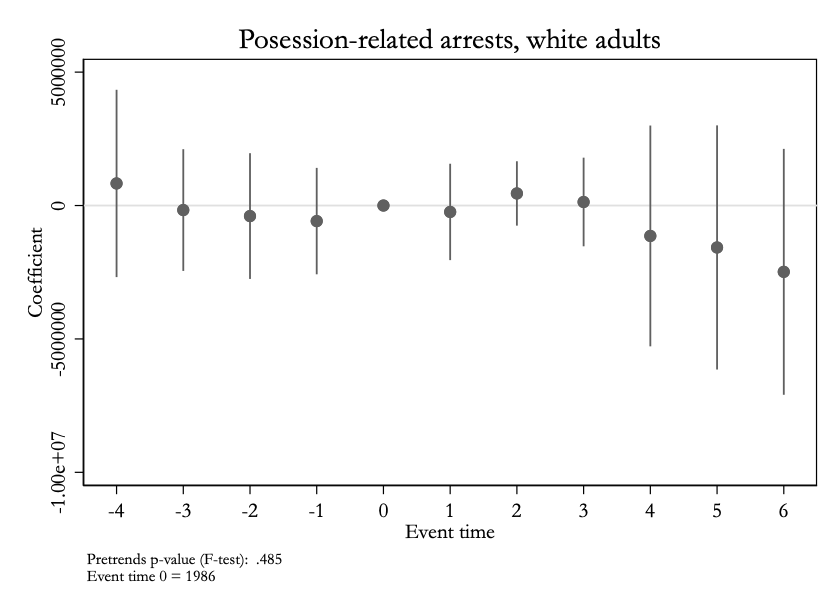
\includegraphics[width=5cm]{eventstudy_white.png} }}%
    \caption{Treatment: states that increased the punitiveness of their laws}%
    \label{fig:example}%
\end{figure}

Model: $Y_{it}=\phi_{i}+\lambda_{t}+\sum_{s\neq1986}1[t=s]\times treatment_{i}\times\beta_{s}+\epsilon_{is}$

\end{frame}

%------------------------------------------------------------


\end{document}